\chapter{Input-Exploration for the Six Trajectories} \label{app:six-trajectories}

This appendix provides more detail on the six SOSAA trajectories from \Cref{txt:six-trajectories}. In particular, it plots the distributions of the SOSAA inputs for each trajectory. For reference, the trajectory maps are also given.

Each map shows the path of the trajectory over the $\geq 5$ days before it arrives at the SMEAR II measurement station at Hyyti\"al\"a, Finland \cite{smear-station-2013}. While SOSAA simulates $\geq 7$ days of the trajectory, the initial 48-hour warm-up period is excluded from the analysis. The main trajectory has a black outline and is coloured from white at the start over blue and purple to red at the time of arrival in Hyyti\"al\"a. In addition to this main trajectory, six temporally adjacent trajectories are plotted with thinner lines. Specifically, for a trajectory at time $t$, the trajectories at times $t-4\text{h}$, $t-2\text{h}$, $t-1\text{h}$, $t+1\text{h}$, $t+2\text{h}$, and $t+4\text{h}$ are plotted in blue, purple, orange, and yellow. All temporally adjacent paths should roughly line if the meteorological conditions are stable. In contrast, the trajectory that arrived in Hyyti\"al\"a on 23.05.2018 at 13:00 UTC rapidly evolved over the next four hours.

\begin{figure}[H]
    \centering
    \begin{subfigure}
        \centering
        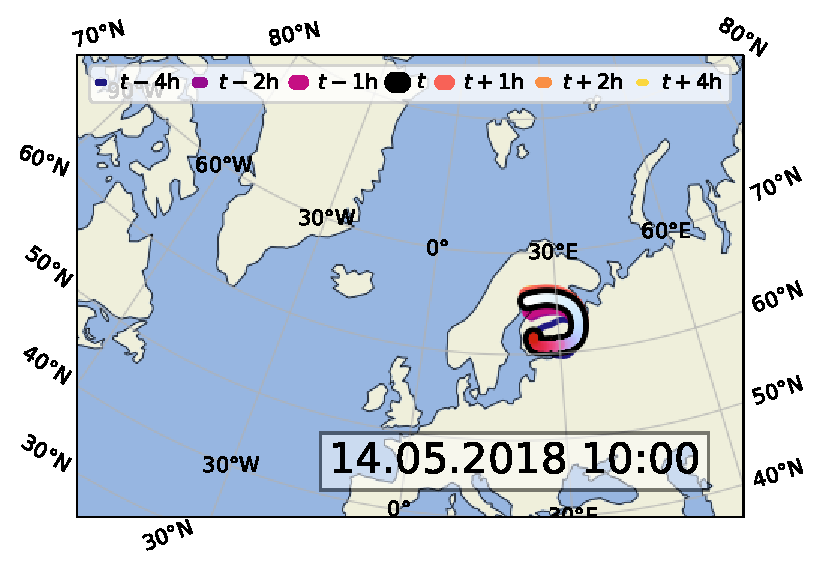
\includegraphics[width=0.32\textwidth,valign=t]{sosaa-data/figures/trajectories/trajectory-14.05.2018:10.00.pdf}
    \end{subfigure}
    \begin{subfigure}
        \centering
        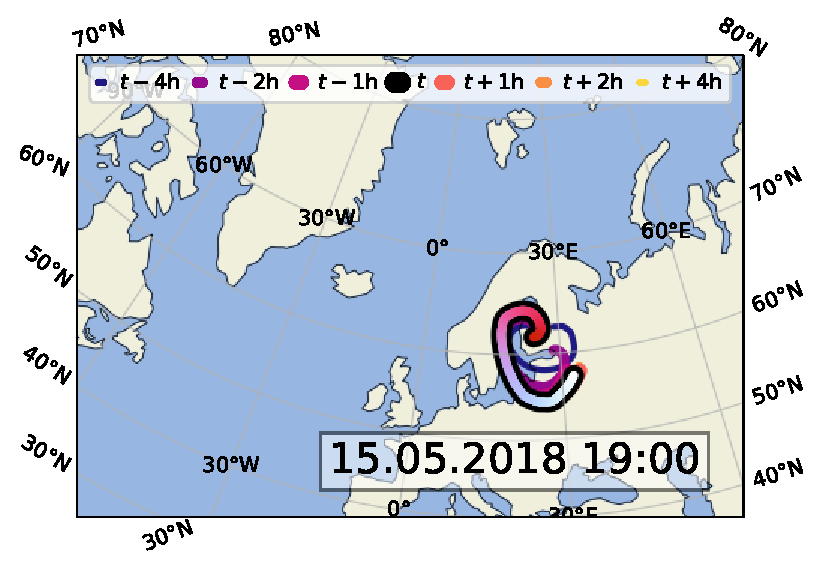
\includegraphics[width=0.32\textwidth,valign=t]{sosaa-data/figures/trajectories/trajectory-15.05.2018:19.00.pdf}
    \end{subfigure}
    \begin{subfigure}
        \centering
        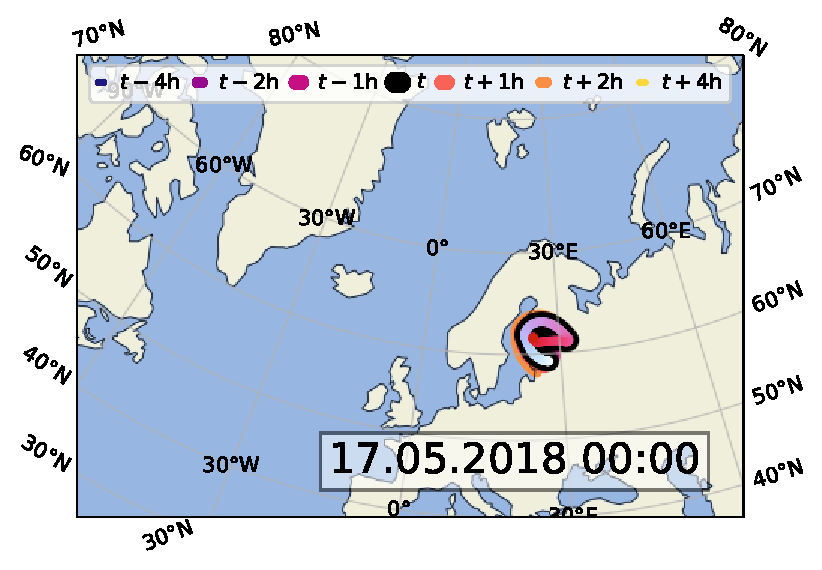
\includegraphics[width=0.32\textwidth,valign=t]{sosaa-data/figures/trajectories/trajectory-17.05.2018:00.00.pdf}
    \end{subfigure}

    \begin{subfigure}
        \centering
        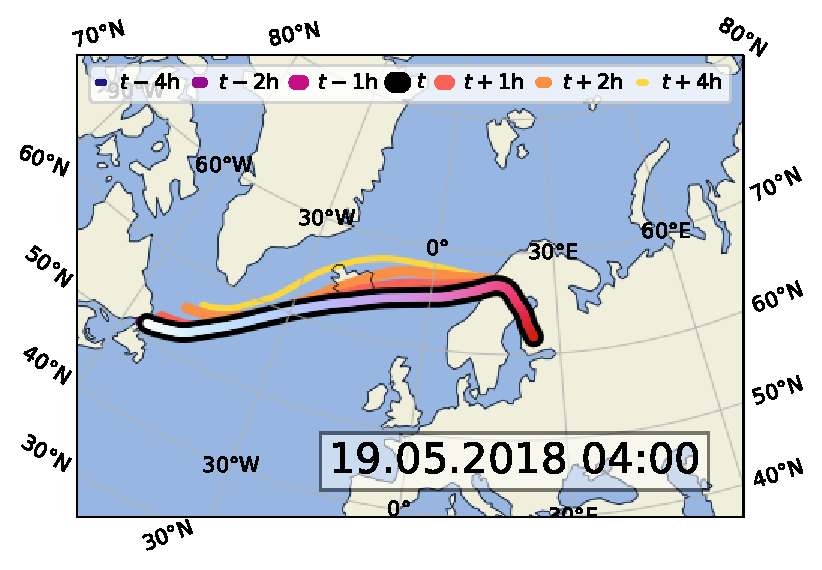
\includegraphics[width=0.32\textwidth,valign=t]{sosaa-data/figures/trajectories/trajectory-19.05.2018:04.00.pdf}
    \end{subfigure}
    \begin{subfigure}
        \centering
        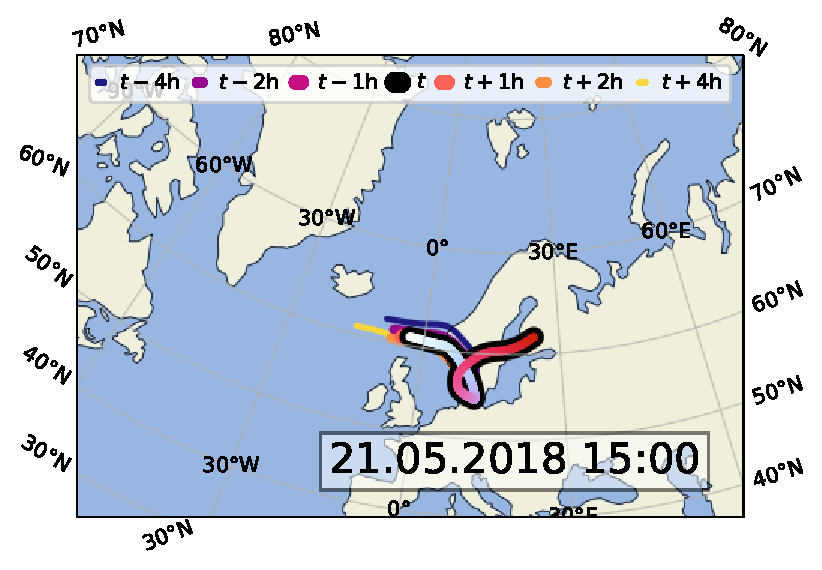
\includegraphics[width=0.32\textwidth,valign=t]{sosaa-data/figures/trajectories/trajectory-21.05.2018:15.00.pdf}
    \end{subfigure}
    \begin{subfigure}
        \centering
        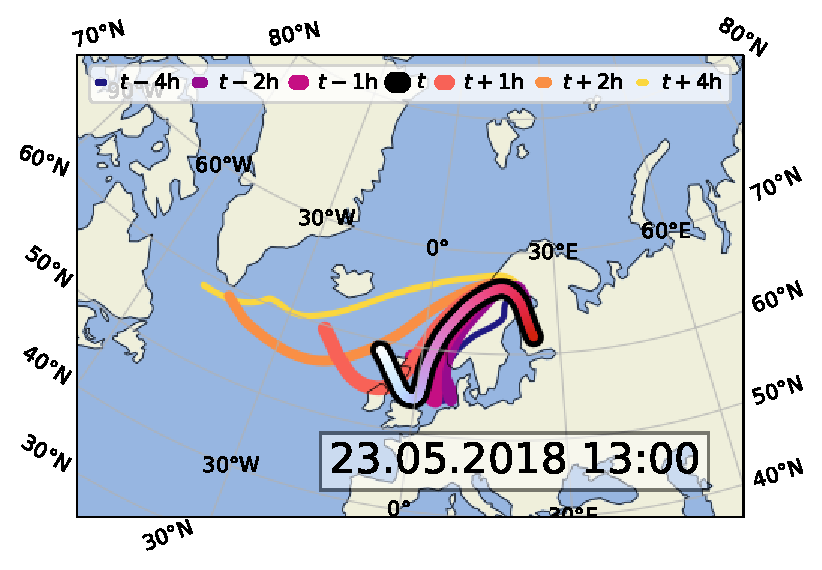
\includegraphics[width=0.32\textwidth,valign=t]{sosaa-data/figures/trajectories/trajectory-23.05.2018:13.00.pdf}
    \end{subfigure}

    \caption[Maps for the six example trajectories]{Maps for the six example trajectories. Each map shows the time-coloured (see \Cref{fig:six-trajectories-ccn}) path of the trajectory that arrives at the listed time in Hyyti\"al\"a, as well as the paths of the prior and next trajectories.}
    \label{fig:six-trajectories-maps-v2}
\end{figure}

\noindent For each trajectory, a graphical summary of the temporal distribution of the emissions and meteorological conditions that are given to SOSAA as inputs is also provided. They are grouped into the eight perturbation categories from \Cref{txt:perturbation-generalisation} that cover aerosol emissions, biogenic emissions, anthropogenic emissions, and air temperature. The input data for each trajectory is shown in a violin plot. Violin plots approximate the probability density function of a distribution using kernel density estimation (see \Cref{eq:kernel-density}) and plot the resulting relative frequency (on the x-axis) against the quantity of interest (on the y-axis). Violin plots are mirrored along the y-axis and often produce visually pleasing shapes. In the following visualisations, scatter plots of the data points are embedded within the violin plots: a random subset of all data points is randomly scattered within the violin body at its respective y-position and coloured according to the time during the trajectory from which this data point comes. Thus, the plots show both the probability and temporal distribution of the inputs.

\begin{figure}[H]
    \centering
    \begin{subfigure}
        \centering
        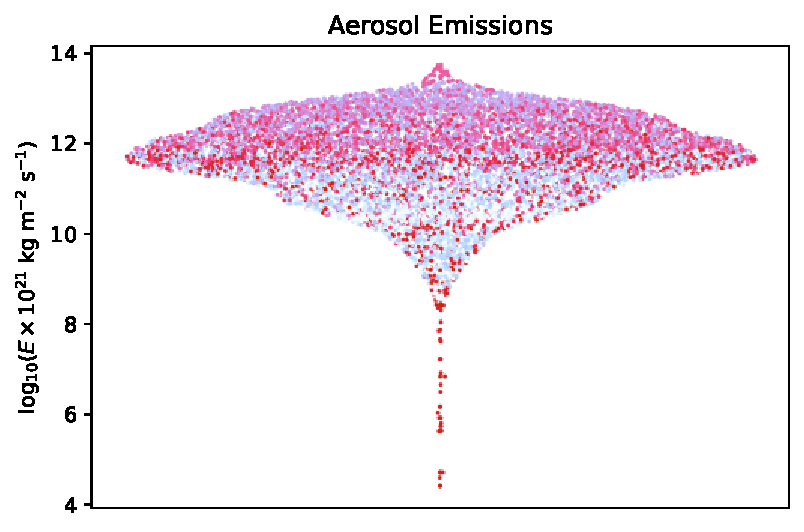
\includegraphics[width=0.49\textwidth,valign=t]{sosaa-data/figures/trajectories/trajectory-14.05.2018:10.00-aerosols.pdf}
    \end{subfigure}
    \begin{subfigure}
        \centering
        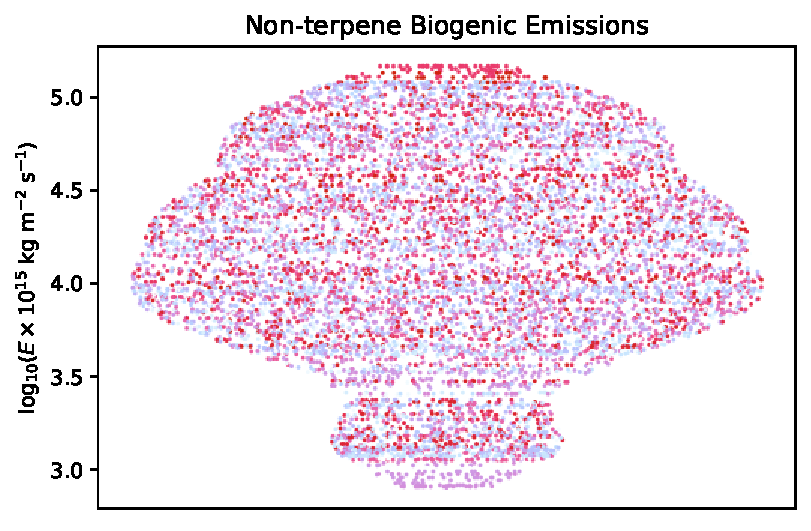
\includegraphics[width=0.49\textwidth,valign=t]{sosaa-data/figures/trajectories/trajectory-14.05.2018:10.00-biogenic.pdf}
    \end{subfigure}
    
    \begin{subfigure}
        \centering
        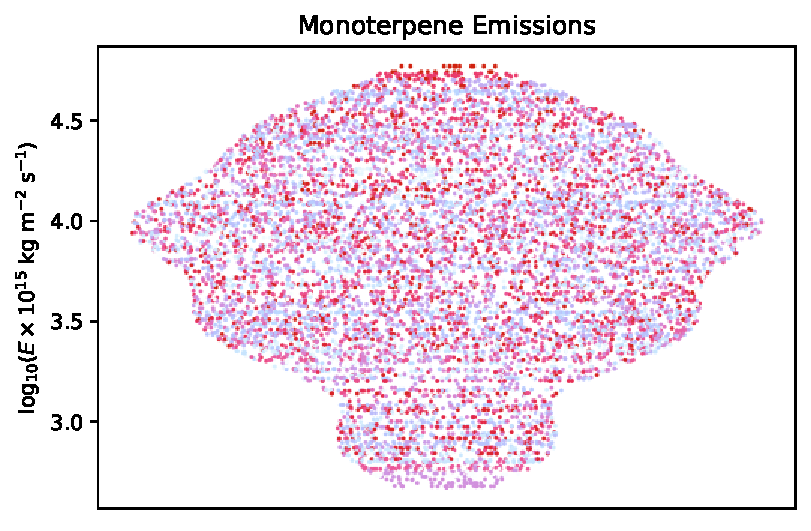
\includegraphics[width=0.49\textwidth,valign=t]{sosaa-data/figures/trajectories/trajectory-14.05.2018:10.00-monoterpenes.pdf}
    \end{subfigure}
    \begin{subfigure}
        \centering
        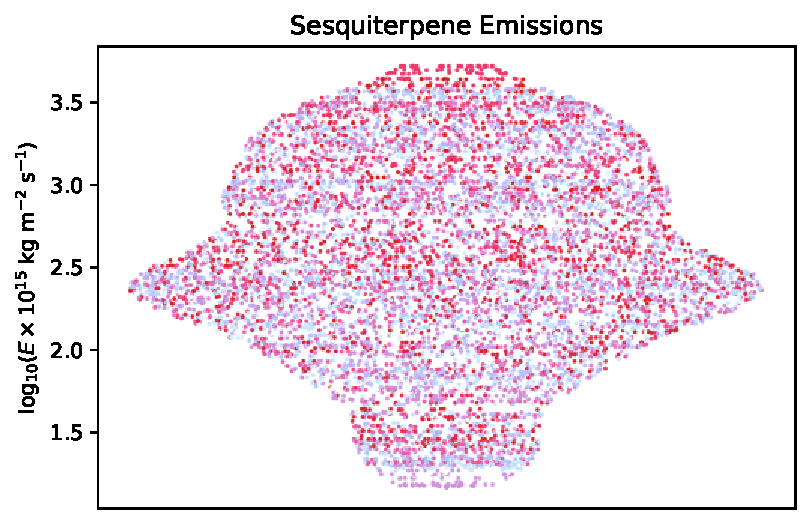
\includegraphics[width=0.49\textwidth,valign=t]{sosaa-data/figures/trajectories/trajectory-14.05.2018:10.00-sesquiterpenes.pdf}
    \end{subfigure}

    \begin{subfigure}
        \centering
        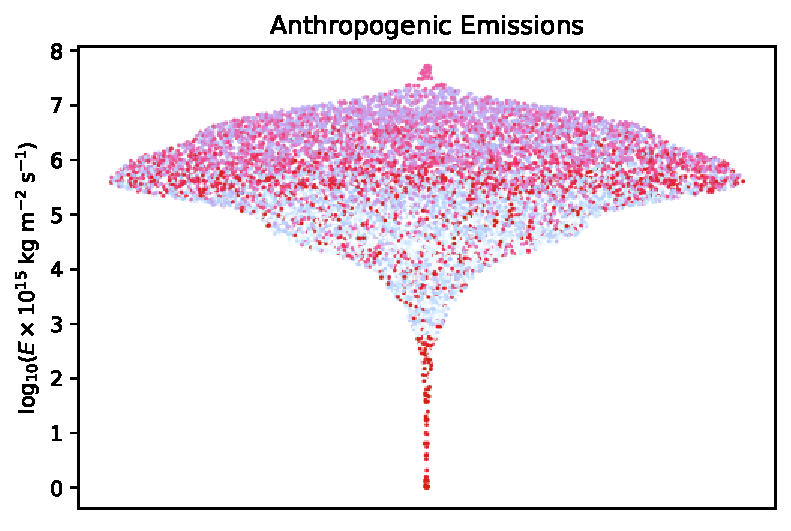
\includegraphics[width=0.49\textwidth,valign=t]{sosaa-data/figures/trajectories/trajectory-14.05.2018:10.00-anthropogenic.pdf}
    \end{subfigure}
    \begin{subfigure}
        \centering
        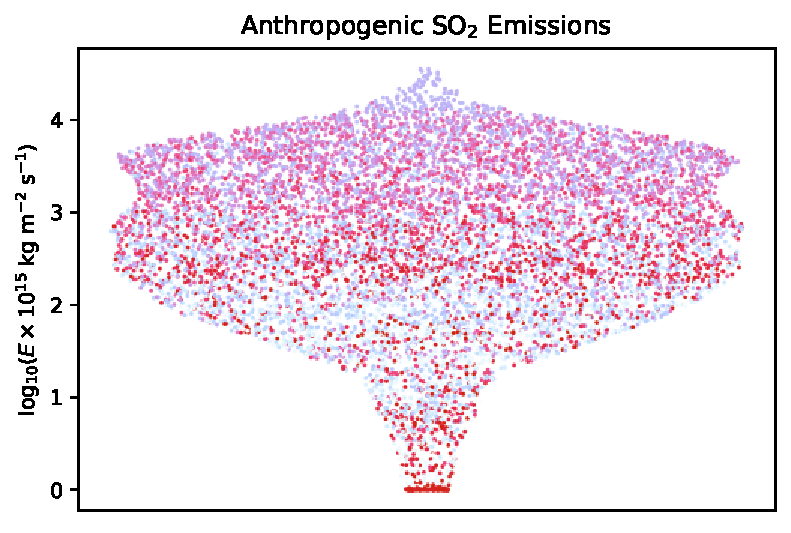
\includegraphics[width=0.49\textwidth,valign=t]{sosaa-data/figures/trajectories/trajectory-14.05.2018:10.00-so2.pdf}
    \end{subfigure}

    \begin{subfigure}
        \centering
        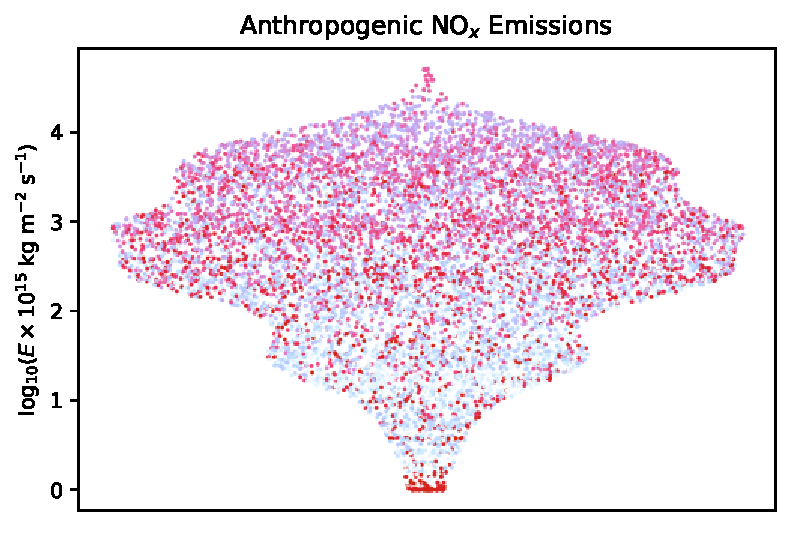
\includegraphics[width=0.49\textwidth,valign=t]{sosaa-data/figures/trajectories/trajectory-14.05.2018:10.00-nox.pdf}
    \end{subfigure}
    \begin{subfigure}
        \centering
        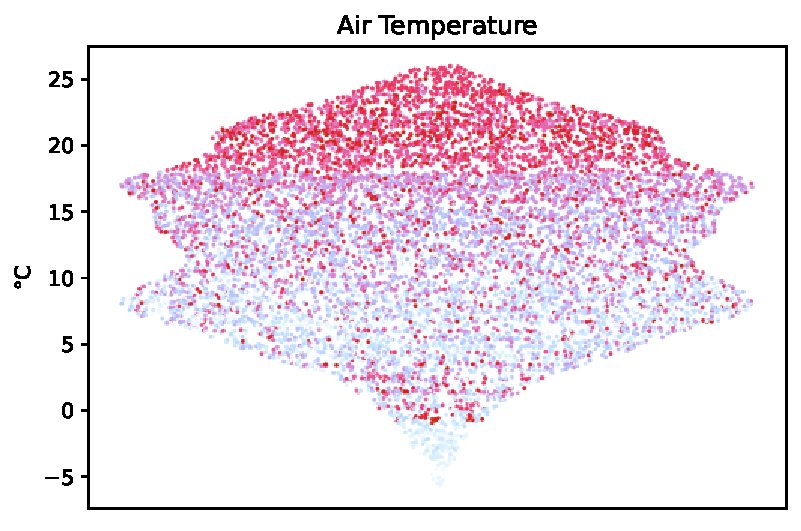
\includegraphics[width=0.49\textwidth,valign=t]{sosaa-data/figures/trajectories/trajectory-14.05.2018:10.00-temperature.pdf}
    \end{subfigure}

    \caption[Inputs for the 14.05.2018 10:00 UTC Trajectory]{SOSAA input distributions for the 14.05.2018 10:00 UTC trajectory (see \Cref{fig:six-trajectories-maps-v2}).}
    \label{fig:trajectory-inputs-14-05}
\end{figure}

\begin{figure}[H]
    \centering
    \begin{subfigure}
        \centering
        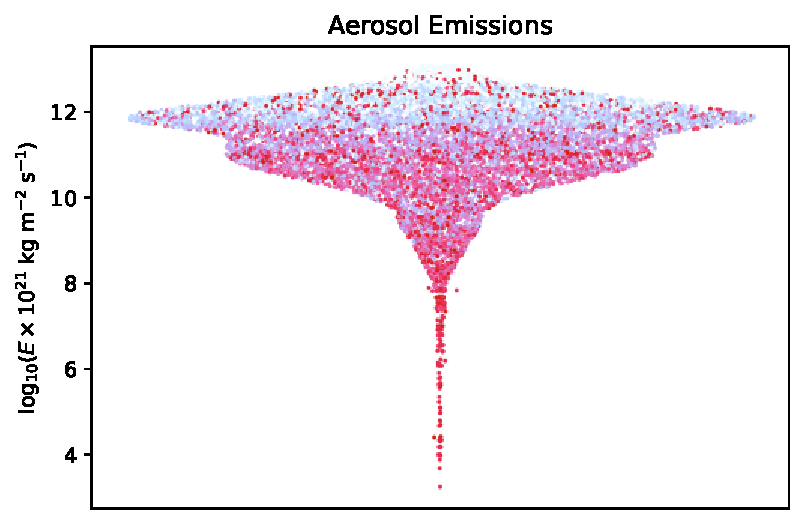
\includegraphics[width=0.49\textwidth,valign=t]{sosaa-data/figures/trajectories/trajectory-15.05.2018:19.00-aerosols.pdf}
    \end{subfigure}
    \begin{subfigure}
        \centering
        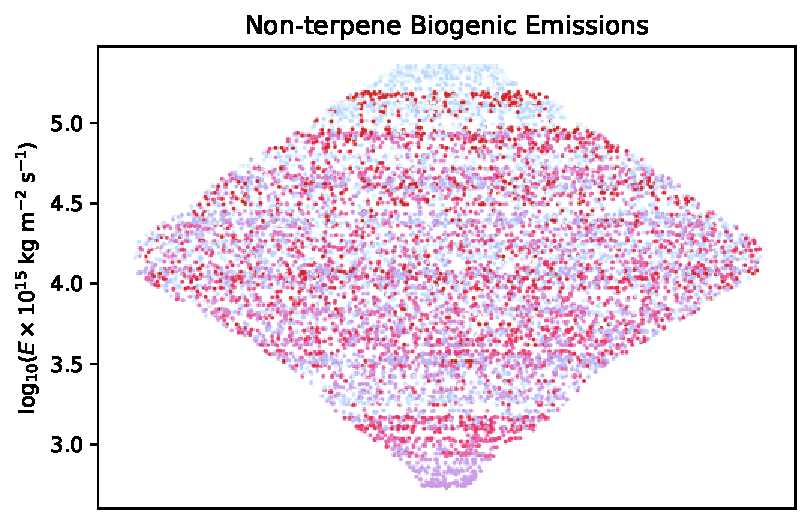
\includegraphics[width=0.49\textwidth,valign=t]{sosaa-data/figures/trajectories/trajectory-15.05.2018:19.00-biogenic.pdf}
    \end{subfigure}
    
    \begin{subfigure}
        \centering
        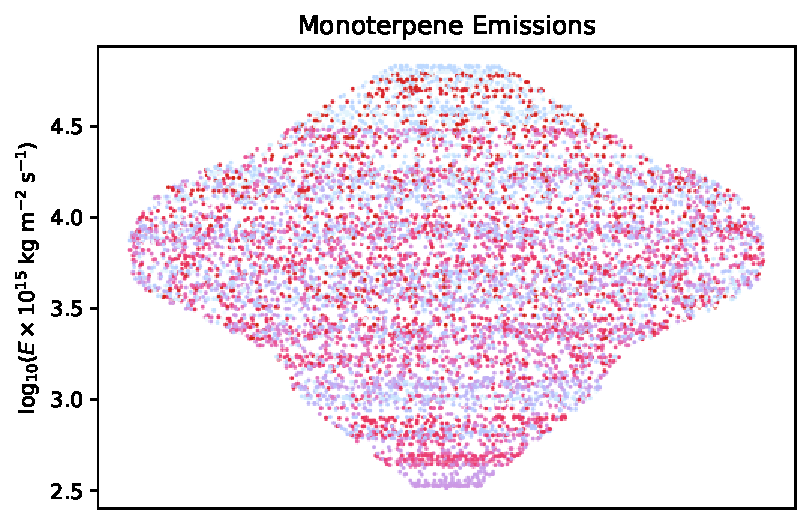
\includegraphics[width=0.49\textwidth,valign=t]{sosaa-data/figures/trajectories/trajectory-15.05.2018:19.00-monoterpenes.pdf}
    \end{subfigure}
    \begin{subfigure}
        \centering
        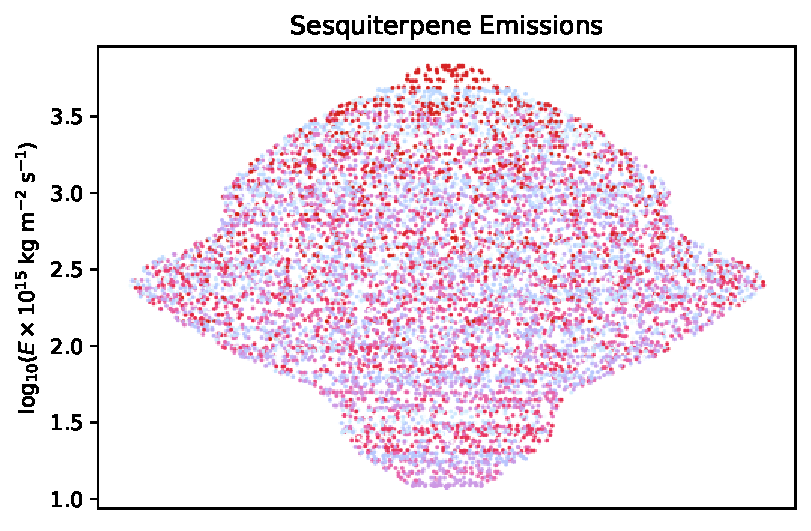
\includegraphics[width=0.49\textwidth,valign=t]{sosaa-data/figures/trajectories/trajectory-15.05.2018:19.00-sesquiterpenes.pdf}
    \end{subfigure}

    \begin{subfigure}
        \centering
        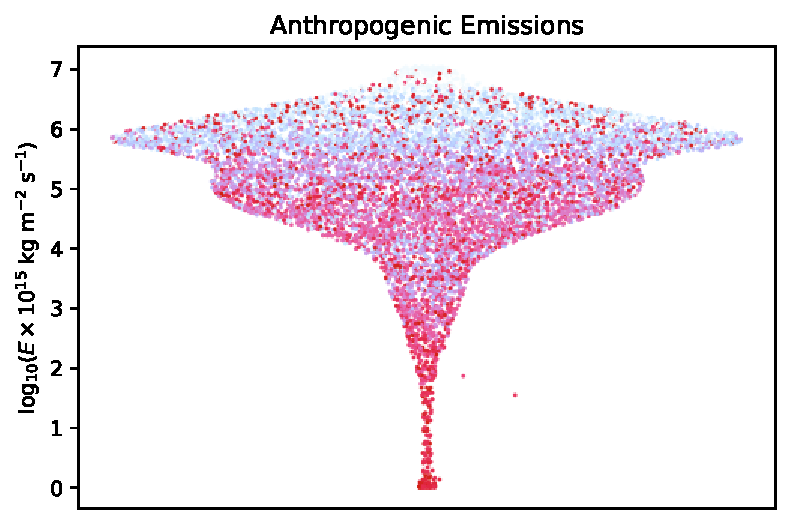
\includegraphics[width=0.49\textwidth,valign=t]{sosaa-data/figures/trajectories/trajectory-15.05.2018:19.00-anthropogenic.pdf}
    \end{subfigure}
    \begin{subfigure}
        \centering
        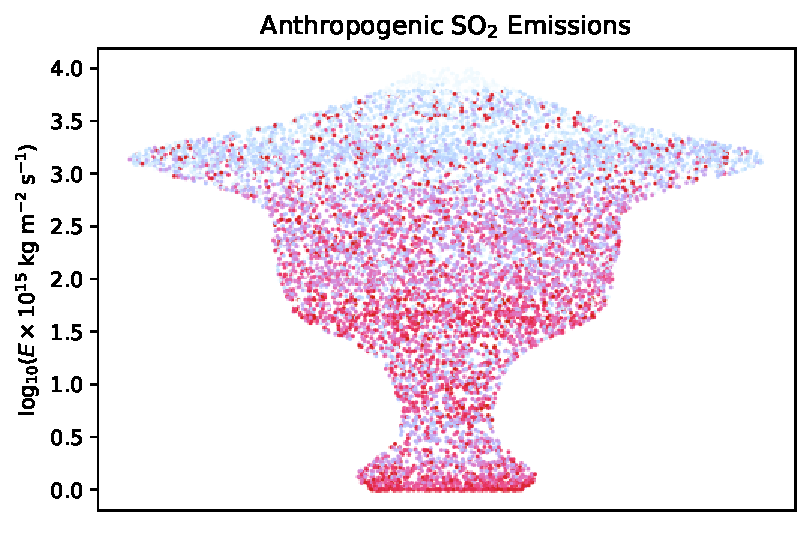
\includegraphics[width=0.49\textwidth,valign=t]{sosaa-data/figures/trajectories/trajectory-15.05.2018:19.00-so2.pdf}
    \end{subfigure}

    \begin{subfigure}
        \centering
        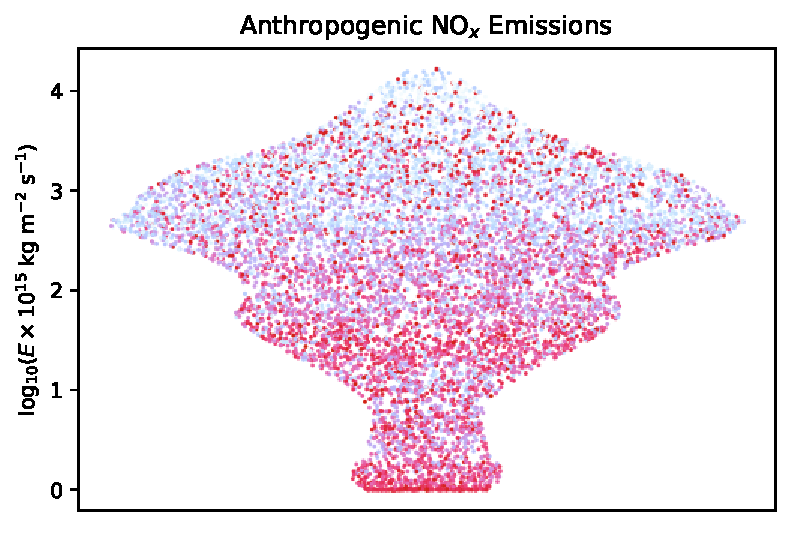
\includegraphics[width=0.49\textwidth,valign=t]{sosaa-data/figures/trajectories/trajectory-15.05.2018:19.00-nox.pdf}
    \end{subfigure}
    \begin{subfigure}
        \centering
        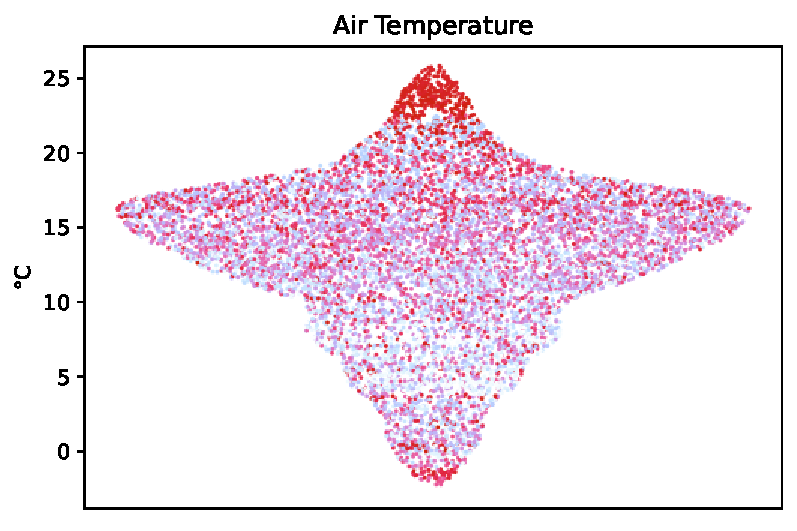
\includegraphics[width=0.49\textwidth,valign=t]{sosaa-data/figures/trajectories/trajectory-15.05.2018:19.00-temperature.pdf}
    \end{subfigure}

    \caption[Inputs for the 15.05.2018 19:00 UTC Trajectory]{SOSAA input distributions for the 15.05.2018 19:00 UTC trajectory (see \Cref{fig:six-trajectories-maps-v2}).}
    \label{fig:trajectory-inputs-15-05}
\end{figure}

\begin{figure}[H]
    \centering
    \begin{subfigure}
        \centering
        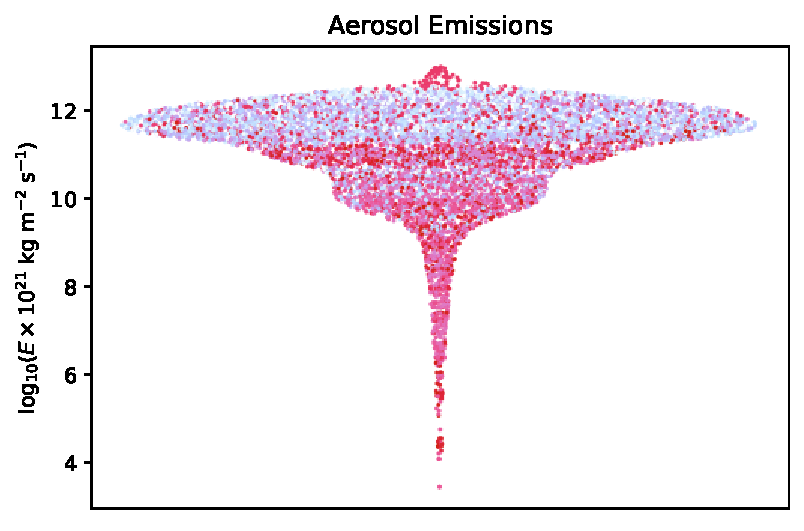
\includegraphics[width=0.49\textwidth,valign=t]{sosaa-data/figures/trajectories/trajectory-17.05.2018:00.00-aerosols.pdf}
    \end{subfigure}
    \begin{subfigure}
        \centering
        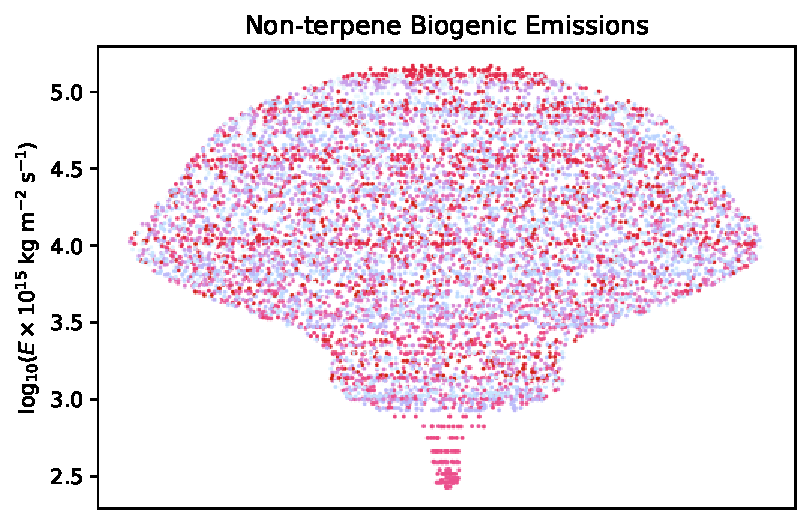
\includegraphics[width=0.49\textwidth,valign=t]{sosaa-data/figures/trajectories/trajectory-17.05.2018:00.00-biogenic.pdf}
    \end{subfigure}
    
    \begin{subfigure}
        \centering
        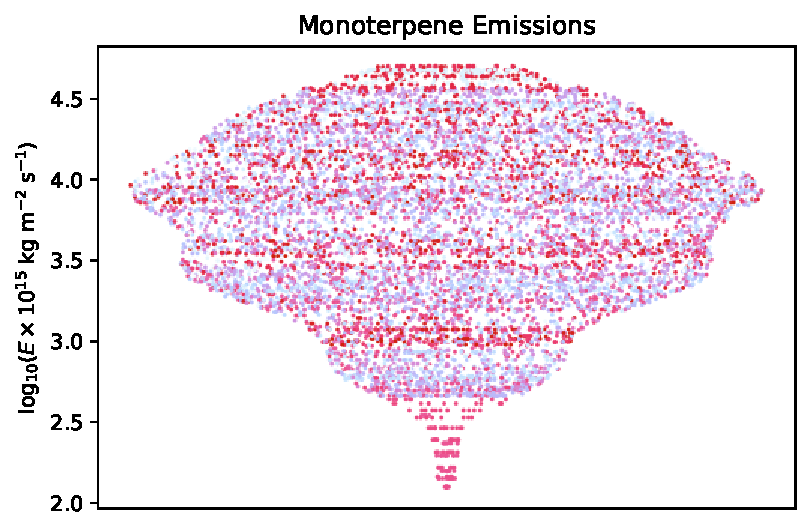
\includegraphics[width=0.49\textwidth,valign=t]{sosaa-data/figures/trajectories/trajectory-17.05.2018:00.00-monoterpenes.pdf}
    \end{subfigure}
    \begin{subfigure}
        \centering
        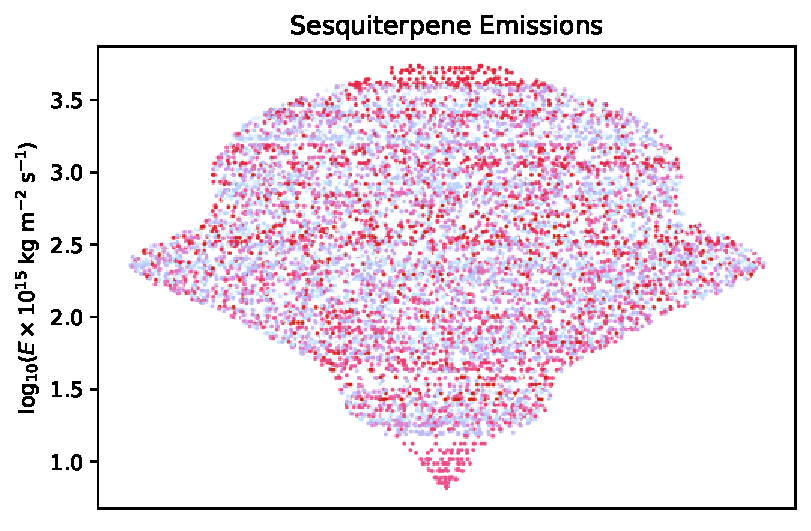
\includegraphics[width=0.49\textwidth,valign=t]{sosaa-data/figures/trajectories/trajectory-17.05.2018:00.00-sesquiterpenes.pdf}
    \end{subfigure}

    \begin{subfigure}
        \centering
        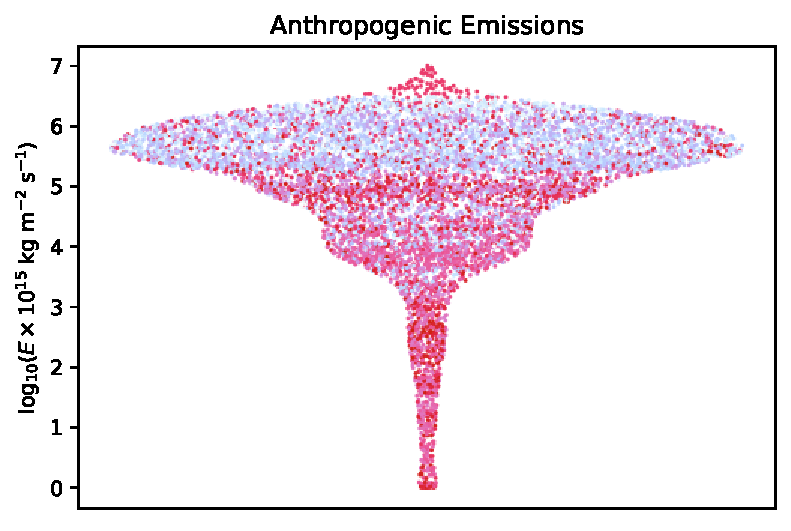
\includegraphics[width=0.49\textwidth,valign=t]{sosaa-data/figures/trajectories/trajectory-17.05.2018:00.00-anthropogenic.pdf}
    \end{subfigure}
    \begin{subfigure}
        \centering
        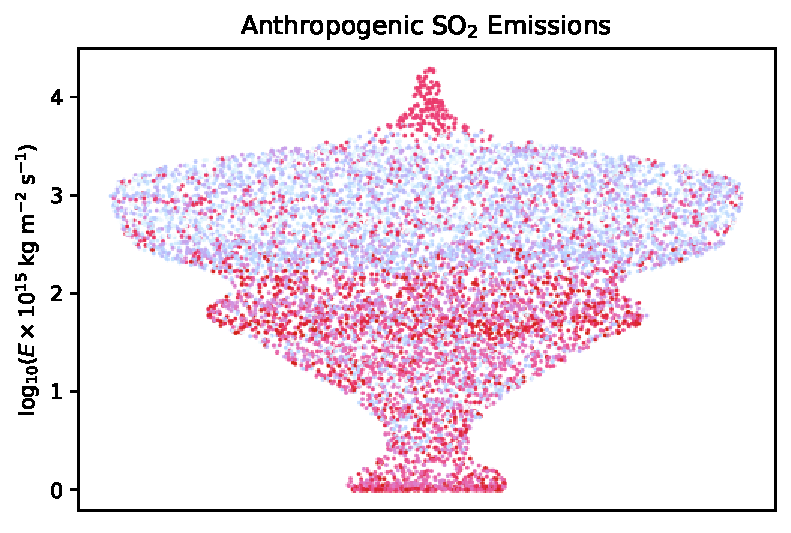
\includegraphics[width=0.49\textwidth,valign=t]{sosaa-data/figures/trajectories/trajectory-17.05.2018:00.00-so2.pdf}
    \end{subfigure}

    \begin{subfigure}
        \centering
        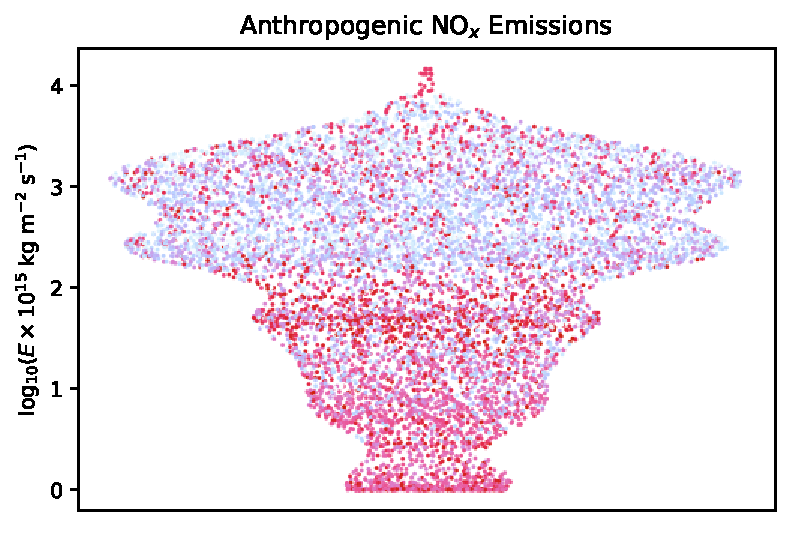
\includegraphics[width=0.49\textwidth,valign=t]{sosaa-data/figures/trajectories/trajectory-17.05.2018:00.00-nox.pdf}
    \end{subfigure}
    \begin{subfigure}
        \centering
        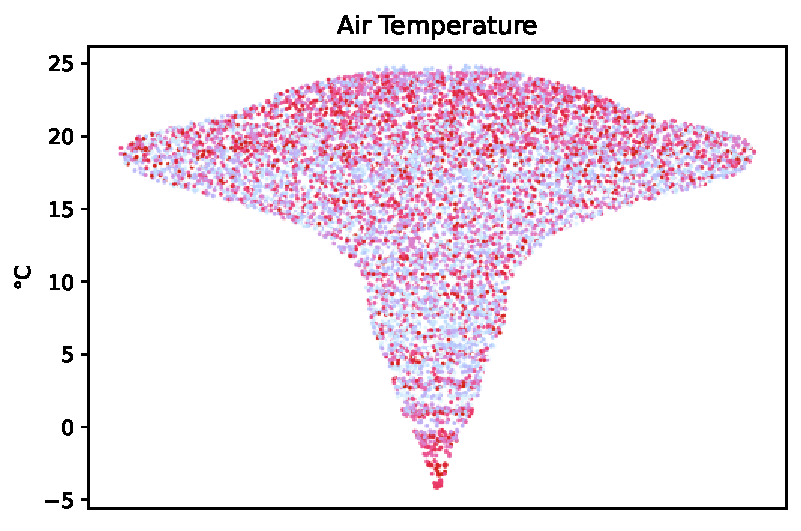
\includegraphics[width=0.49\textwidth,valign=t]{sosaa-data/figures/trajectories/trajectory-17.05.2018:00.00-temperature.pdf}
    \end{subfigure}

    \caption[Inputs for the 17.05.2018 00:00 UTC Trajectory]{SOSAA input distributions for the 17.05.2018 00:00 UTC trajectory (see \Cref{fig:six-trajectories-maps-v2}).}
    \label{fig:trajectory-inputs-17-05}
\end{figure}

\begin{figure}[H]
    \centering
    \begin{subfigure}
        \centering
        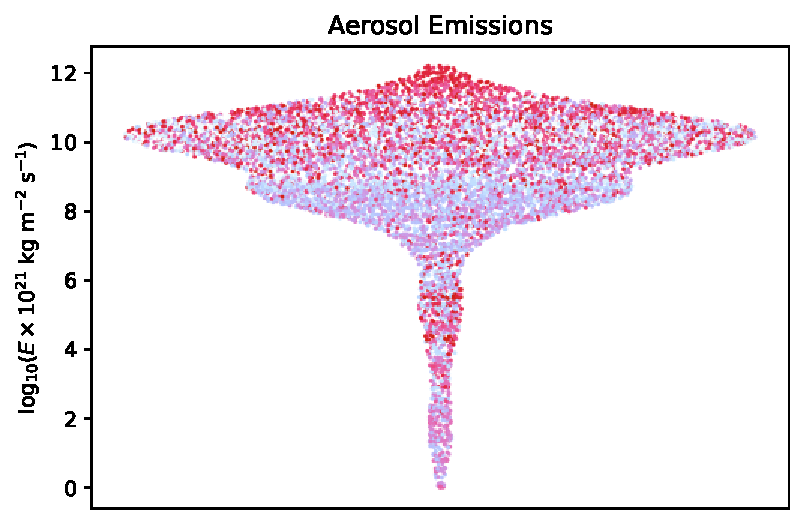
\includegraphics[width=0.49\textwidth,valign=t]{sosaa-data/figures/trajectories/trajectory-19.05.2018:04.00-aerosols.pdf}
    \end{subfigure}
    \begin{subfigure}
        \centering
        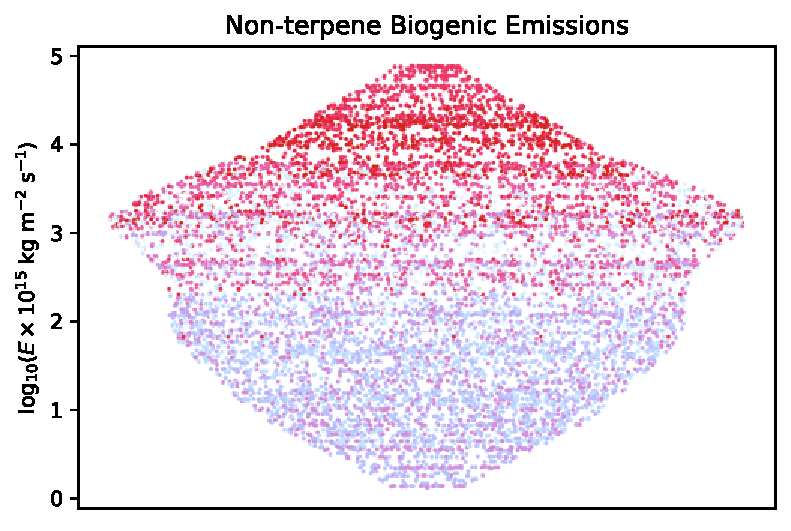
\includegraphics[width=0.49\textwidth,valign=t]{sosaa-data/figures/trajectories/trajectory-19.05.2018:04.00-biogenic.pdf}
    \end{subfigure}
    
    \begin{subfigure}
        \centering
        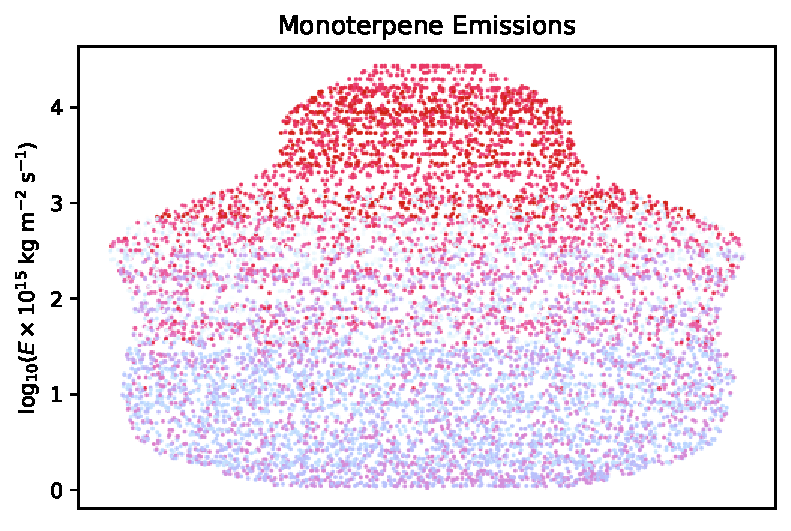
\includegraphics[width=0.49\textwidth,valign=t]{sosaa-data/figures/trajectories/trajectory-19.05.2018:04.00-monoterpenes.pdf}
    \end{subfigure}
    \begin{subfigure}
        \centering
        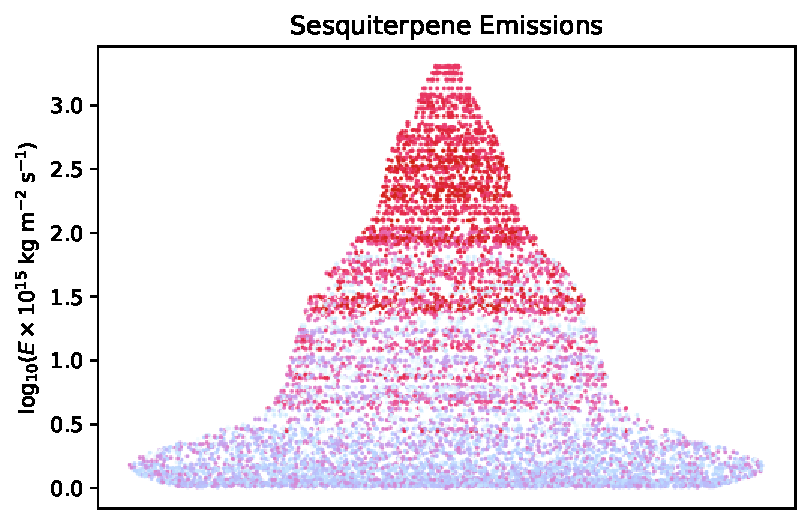
\includegraphics[width=0.49\textwidth,valign=t]{sosaa-data/figures/trajectories/trajectory-19.05.2018:04.00-sesquiterpenes.pdf}
    \end{subfigure}

    \begin{subfigure}
        \centering
        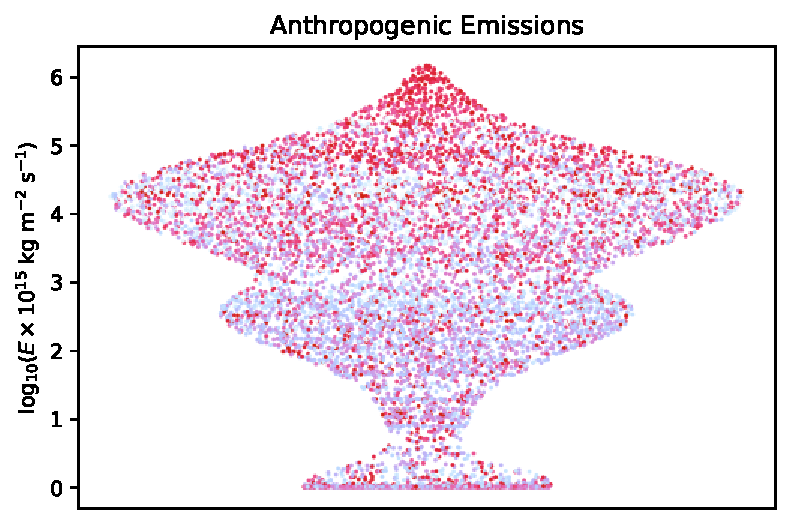
\includegraphics[width=0.49\textwidth,valign=t]{sosaa-data/figures/trajectories/trajectory-19.05.2018:04.00-anthropogenic.pdf}
    \end{subfigure}
    \begin{subfigure}
        \centering
        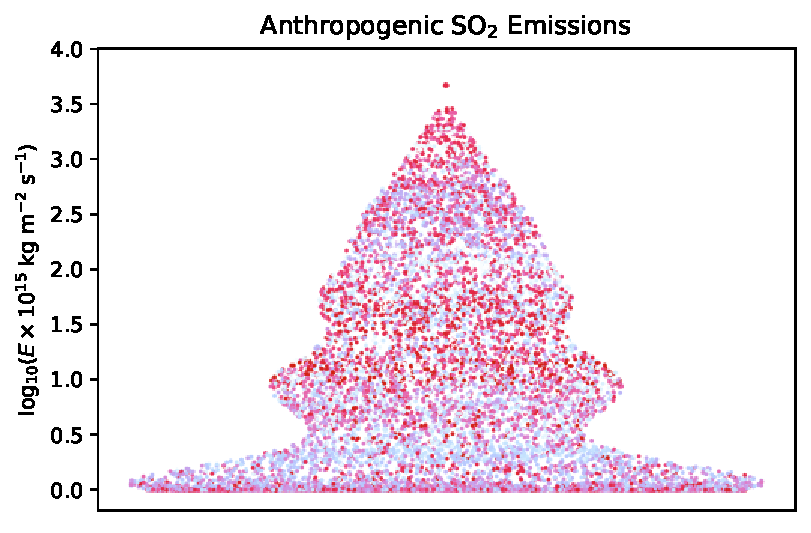
\includegraphics[width=0.49\textwidth,valign=t]{sosaa-data/figures/trajectories/trajectory-19.05.2018:04.00-so2.pdf}
    \end{subfigure}

    \begin{subfigure}
        \centering
        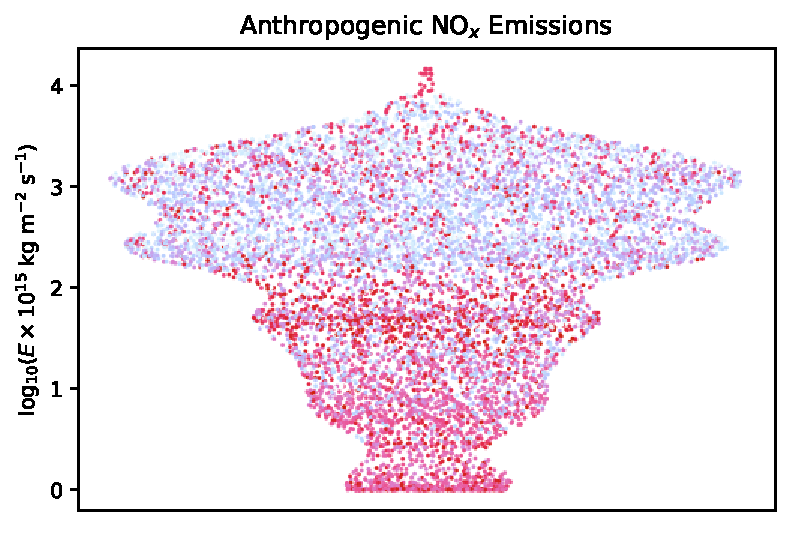
\includegraphics[width=0.49\textwidth,valign=t]{sosaa-data/figures/trajectories/trajectory-17.05.2018:00.00-nox.pdf}
    \end{subfigure}
    \begin{subfigure}
        \centering
        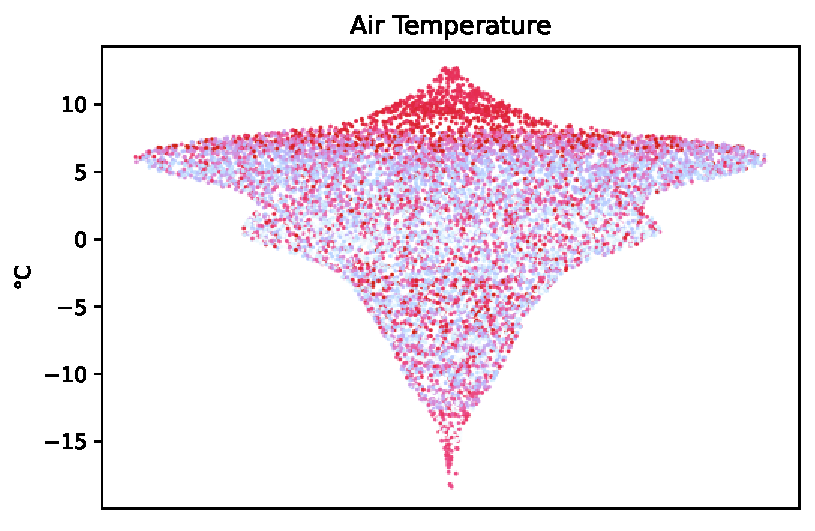
\includegraphics[width=0.49\textwidth,valign=t]{sosaa-data/figures/trajectories/trajectory-19.05.2018:04.00-temperature.pdf}
    \end{subfigure}

    \caption[Inputs for the 19.05.2018 04:00 UTC Trajectory]{SOSAA input distributions for the 19.05.2018 04:00 UTC trajectory (see \Cref{fig:six-trajectories-maps-v2}).}
    \label{fig:trajectory-inputs-19-05}
\end{figure}

\begin{figure}[H]
    \centering
    \begin{subfigure}
        \centering
        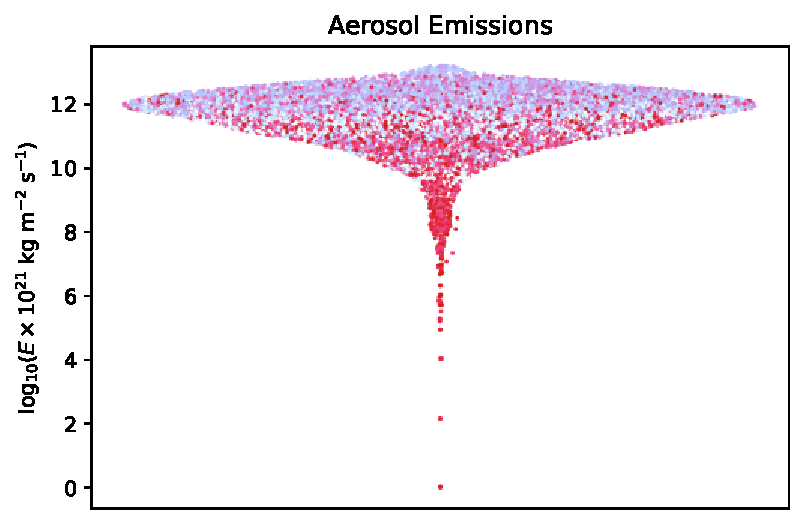
\includegraphics[width=0.49\textwidth,valign=t]{sosaa-data/figures/trajectories/trajectory-21.05.2018:15.00-aerosols.pdf}
    \end{subfigure}
    \begin{subfigure}
        \centering
        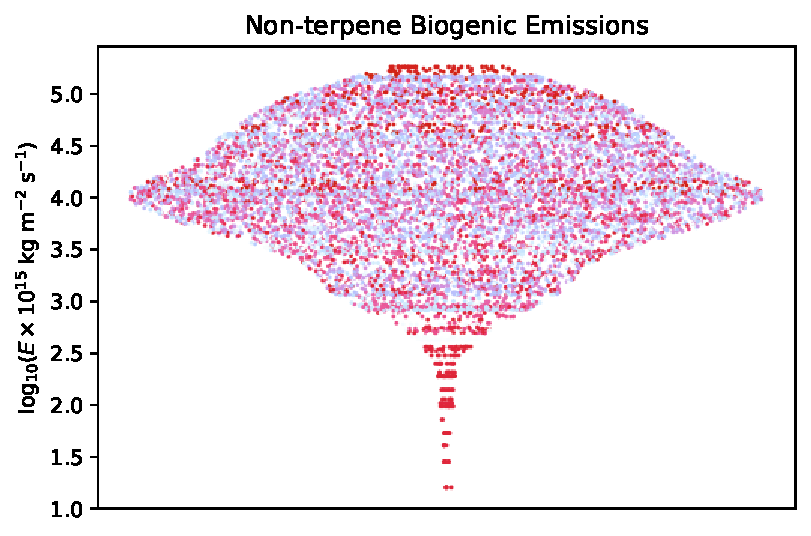
\includegraphics[width=0.49\textwidth,valign=t]{sosaa-data/figures/trajectories/trajectory-21.05.2018:15.00-biogenic.pdf}
    \end{subfigure}
    
    \begin{subfigure}
        \centering
        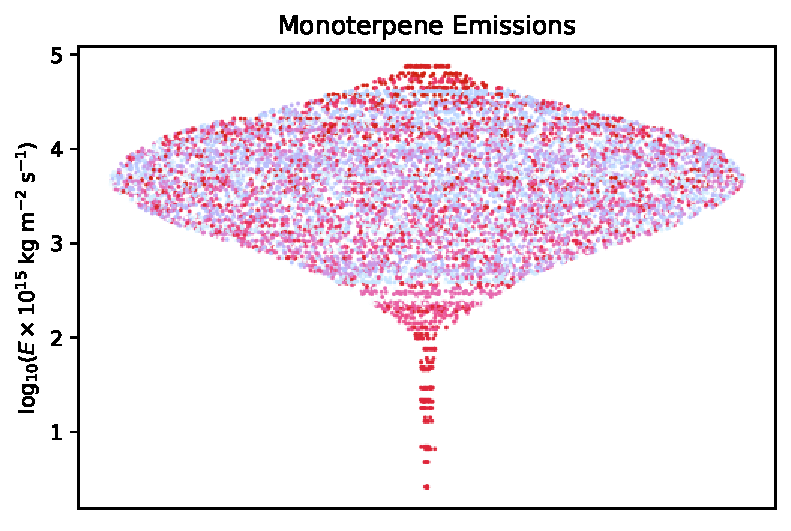
\includegraphics[width=0.49\textwidth,valign=t]{sosaa-data/figures/trajectories/trajectory-21.05.2018:15.00-monoterpenes.pdf}
    \end{subfigure}
    \begin{subfigure}
        \centering
        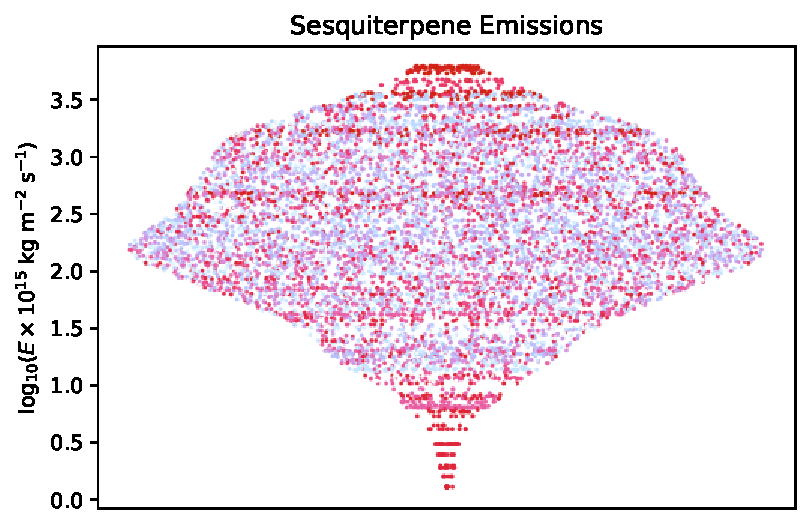
\includegraphics[width=0.49\textwidth,valign=t]{sosaa-data/figures/trajectories/trajectory-21.05.2018:15.00-sesquiterpenes.pdf}
    \end{subfigure}

    \begin{subfigure}
        \centering
        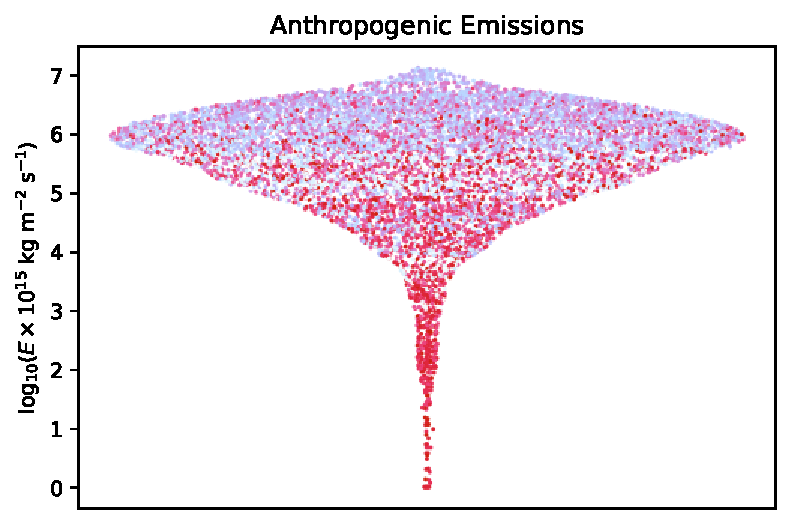
\includegraphics[width=0.49\textwidth,valign=t]{sosaa-data/figures/trajectories/trajectory-21.05.2018:15.00-anthropogenic.pdf}
    \end{subfigure}
    \begin{subfigure}
        \centering
        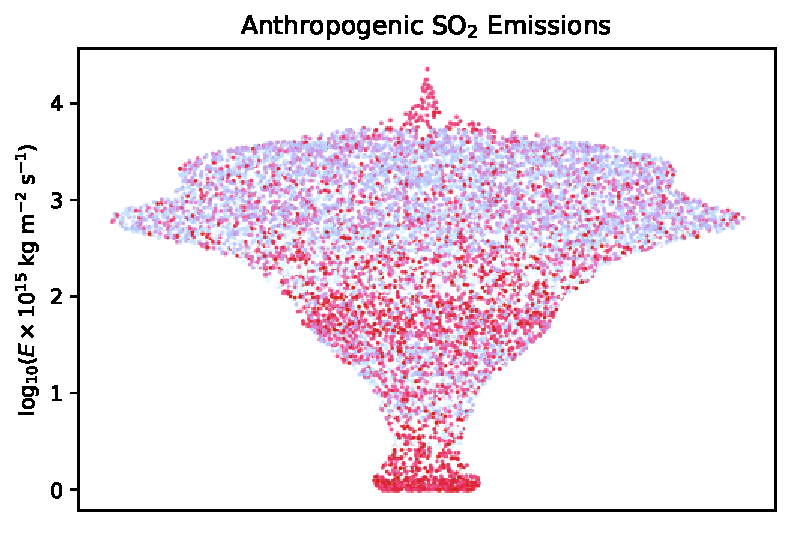
\includegraphics[width=0.49\textwidth,valign=t]{sosaa-data/figures/trajectories/trajectory-21.05.2018:15.00-so2.pdf}
    \end{subfigure}

    \begin{subfigure}
        \centering
        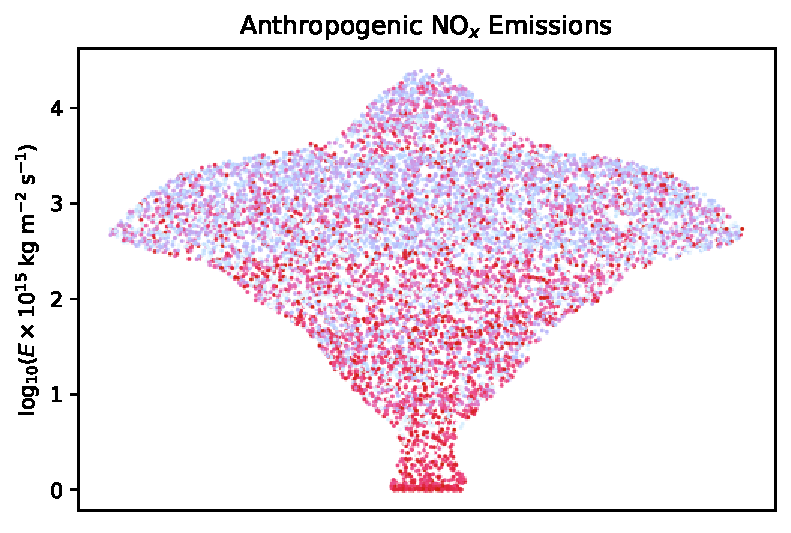
\includegraphics[width=0.49\textwidth,valign=t]{sosaa-data/figures/trajectories/trajectory-21.05.2018:15.00-nox.pdf}
    \end{subfigure}
    \begin{subfigure}
        \centering
        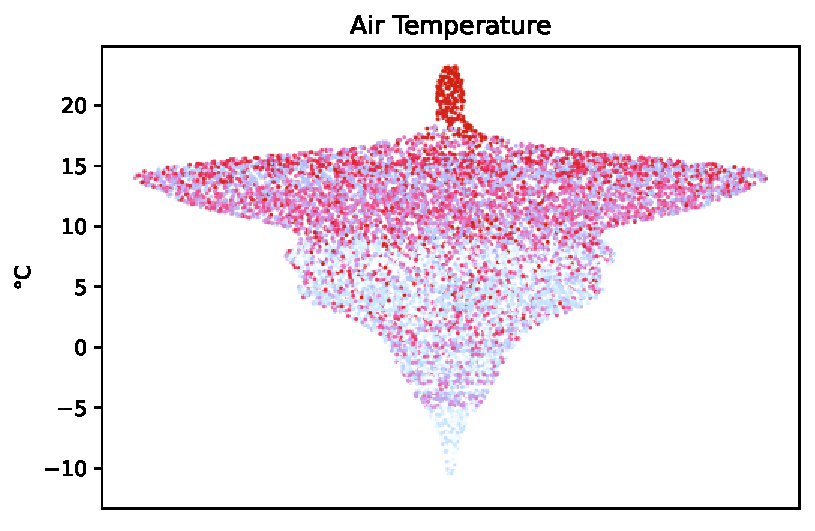
\includegraphics[width=0.49\textwidth,valign=t]{sosaa-data/figures/trajectories/trajectory-21.05.2018:15.00-temperature.pdf}
    \end{subfigure}

    \caption[Inputs for the 21.05.2018 15:00 UTC Trajectory]{SOSAA input distributions for the 21.05.2018 15:00 UTC trajectory (see \Cref{fig:six-trajectories-maps-v2}).}
    \label{fig:trajectory-inputs-21-05}
\end{figure}

\begin{figure}[H]
    \centering
    \begin{subfigure}
        \centering
        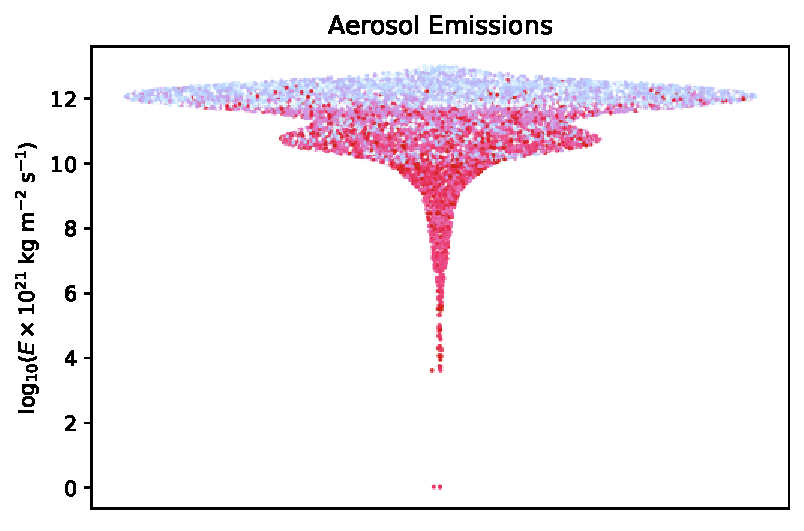
\includegraphics[width=0.49\textwidth,valign=t]{sosaa-data/figures/trajectories/trajectory-23.05.2018:13.00-aerosols.pdf}
    \end{subfigure}
    \begin{subfigure}
        \centering
        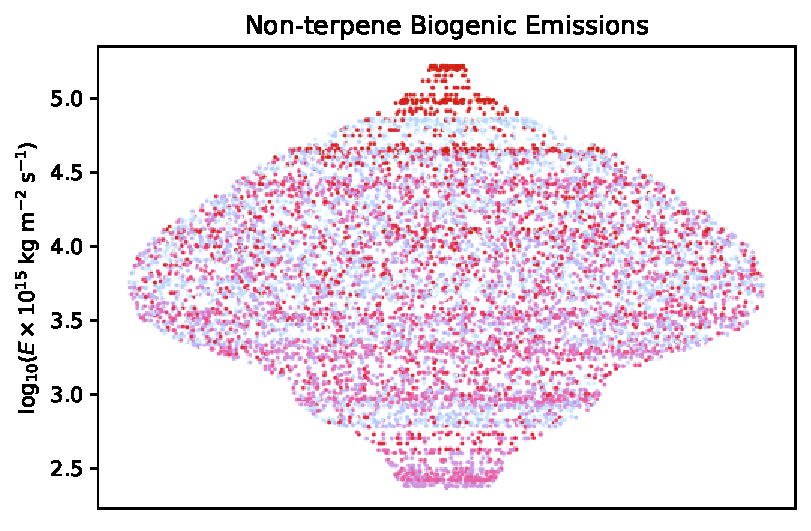
\includegraphics[width=0.49\textwidth,valign=t]{sosaa-data/figures/trajectories/trajectory-23.05.2018:13.00-biogenic.pdf}
    \end{subfigure}
    
    \begin{subfigure}
        \centering
        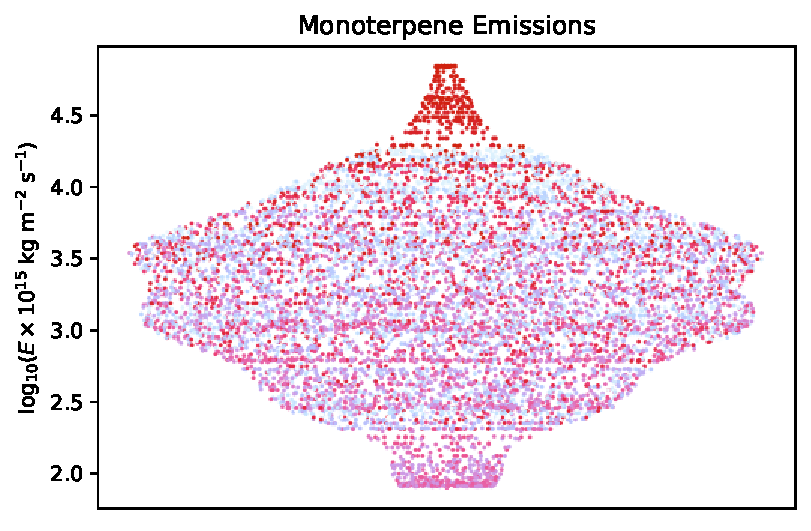
\includegraphics[width=0.49\textwidth,valign=t]{sosaa-data/figures/trajectories/trajectory-23.05.2018:13.00-monoterpenes.pdf}
    \end{subfigure}
    \begin{subfigure}
        \centering
        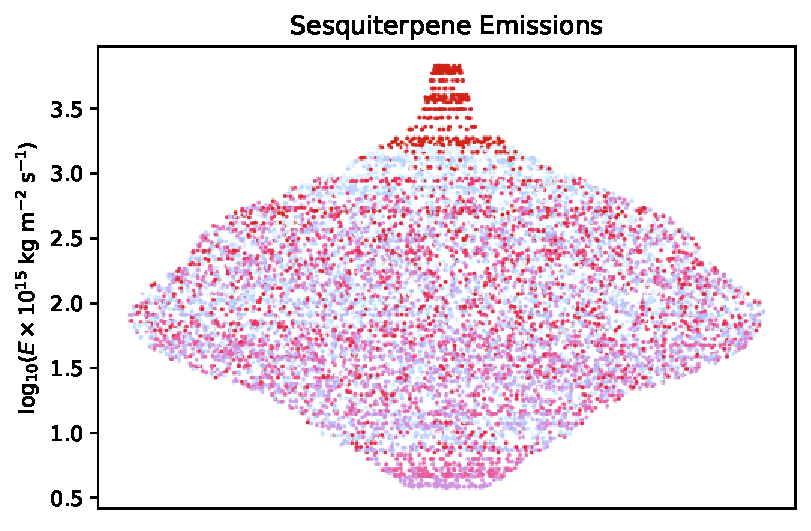
\includegraphics[width=0.49\textwidth,valign=t]{sosaa-data/figures/trajectories/trajectory-23.05.2018:13.00-sesquiterpenes.pdf}
    \end{subfigure}

    \begin{subfigure}
        \centering
        \includegraphics[width=0.49\textwidth,valign=t]{sosaa-data/figures/trajectories/trajectory-23.05.2018:13.00-anthropogenic.pdf}
    \end{subfigure}
    \begin{subfigure}
        \centering
        \includegraphics[width=0.49\textwidth,valign=t]{sosaa-data/figures/trajectories/trajectory-23.05.2018:13.00-so2.pdf}
    \end{subfigure}

    \begin{subfigure}
        \centering
        \includegraphics[width=0.49\textwidth,valign=t]{sosaa-data/figures/trajectories/trajectory-23.05.2018:13.00-nox.pdf}
    \end{subfigure}
    \begin{subfigure}
        \centering
        \includegraphics[width=0.49\textwidth,valign=t]{sosaa-data/figures/trajectories/trajectory-23.05.2018:13.00-temperature.pdf}
    \end{subfigure}

    \caption[Inputs for the 23.05.2018 13:00 UTC Trajectory]{SOSAA input distributions for the 23.05.2018 13:00 UTC trajectory (see \Cref{fig:six-trajectories-maps-v2}).}
    \label{fig:trajectory-inputs-23-05}
\end{figure}
